\documentclass{standalone}
\usepackage{tikz}

\begin{document}

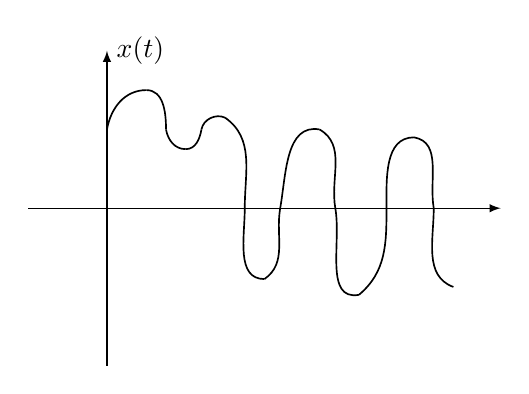
\begin{tikzpicture}[>=latex]
	\draw [->] (-1,0) -- (5,0);
	\draw [->] (0,-2) -- (0,2) node [right] {\(x(t)\)};
	% \node [opacity=0.5] at (1.6,0) {\includegraphics[scale = 0.25]{imagen.png}};

% CURVA
	\begin{scope}[semithick]
		\draw (0,1) to [out=80 , in=180] (0.5,1.5);
		\draw (0.5,1.5) to [out=0 , in=90] (0.75,1);
		\draw (0.75,1) to [out=-80 , in=180] (1,0.75);
		\draw (1,0.75) to [out=0 , in=260] (1.2,1);
		\draw (1.2,1) to [out=80 , in=155] (1.5,1.15);
		\draw (1.5,1.15) to [out=-35 , in=90] (1.75,0);
		\draw (1.75,0) to [out=-90 , in=180] (2,-0.9);
		\draw (2,-0.9) to [out=35 , in=-100] (2.2,0);
		\draw (2.2,0) to [out=80 , in=170] (2.7,1);
		\draw (2.7,1) to [out=-30 , in=100] (2.9,0);
		\draw (2.9,0) to [out=-80 , in=190] (3.2,-1.1);
		\draw (3.2,-1.1) to [out=40 , in=270] (3.55,0);
		\draw (3.55,0) to [out=90 , in=180] (3.9,0.9);
		\draw (3.9,0.9) to [out=-10 , in=100] (4.15,0);
		\draw (4.15,0) to [out=-90 , in=160] (4.4,-1);
	\end{scope}

% PUNTOS
	% \fill (0,1) circle (1.5pt);
	% \fill [red] (0.5,1.5) circle (1.5pt);
	% \fill (0.75,1) circle (1.5pt);
	% \fill [red] (1,0.75) circle (1.5pt);
	% \fill (1.2,1) circle (1.5pt);
	% \fill [red] (1.5,1.15) circle (1.5pt);
	% \fill (1.75,0) circle (1.5pt);
	% \fill [red] (2,-0.9) circle (1.5pt);
	% \fill (2.2,0) circle (1.5pt);
	% \fill [red] (2.7,1) circle (1.5pt);
	% \fill (2.9,0) circle (1.5pt);
	% \fill [red] (3.2,-1.1) circle (1.5pt);
	% \fill (3.55,0) circle (1.5pt);
	% \fill [red] (3.9,0.9) circle (1.5pt);
	% \fill (4.15,0) circle (1.5pt);
	% \fill [red] (4.4,-1) circle (1.5pt);
\end{tikzpicture}

\end{document}
